\documentclass[a4paper,11pt]{beamer}
\usepackage{etex}
\usepackage{lmodern}
\usepackage[french]{babel}
\usepackage[T1]{fontenc}
\usepackage[utf8]{inputenc}
\usepackage{pst-sigsys} 
\usepackage{amsmath,amsfonts,amssymb}
\usepackage{pstricks-add} 
\usepackage{ragged2e}
\usepackage{graphicx}   
\usepackage{ulem} 
\usepackage{wasysym}
\usepackage{matlab-prettifier}
\usepackage{hyperref}
\usepackage{listings}
\usepackage{color}
\setbeamertemplate{navigation symbols}{}   
  
\usetheme{Darmstadt} 
\setbeamertemplate{footline}{\insertframenumber/\inserttotalframenumber}
\title{DOCoMETRe - Installation}
\author{Frank BULOUP - frank.buloup@univ-amu.fr} 
\institute{Aix Marseille Université\\Institut des Sciences du Mouvement}
\date{}

\setbeamertemplate{footline} 
{  
	\begin{beamercolorbox}[ht=2.5ex,dp=1.125ex,%
      leftskip=.3cm,rightskip=.3cm plus1fil]{title in head/foot}%
      {\usebeamerfont{title in head/foot}\insertshorttitle} \hfill    
      \insertframenumber / \inserttotalframenumber%
    \end{beamercolorbox}%
%     \begin{beamercolorbox}[colsep=1.5pt]{lower separation line foot}
%     \end{beamercolorbox} 
}
 
\newcounter{exampleBlockCounter}
\setcounter{exampleBlockCounter}{1} 

% Custom colors
%\definecolor{deepblue}{rgb}{0,0,0.5}
%\definecolor{deepred}{rgb}{0.6,0,0}
%\definecolor{deepgreen}{rgb}{0,0.5,0}
\definecolor{comment}{rgb}{0.12, 0.38, 0.18 } %adjusted, in Eclipse: {0.25, 0.42, 0.30 } = #3F6A4D
\definecolor{keyword}{rgb}{0.37, 0.08, 0.25}  % #5F1441
\definecolor{string}{rgb}{0.06, 0.10, 0.98} % #101AF9

\lstset{
language=Python,
frame=single,
frameround=tttt,
rulesepcolor=\color{black},
showspaces=false,showtabs=false,tabsize=2,
numberstyle=\tiny,numbers=left,
stringstyle=\color{string},
keywordstyle = \color{keyword}\bfseries,
commentstyle=\color{comment}\itshape,
basicstyle=\ttfamily\footnotesize,
breaklines=true,
captionpos=b
}
  
\begin{document} 

\begin{frame}[plain]
	\titlepage
	\center{
\includegraphics[scale=0.75]{images/by-nc-sa.eps}}
	\vspace{1cm}
 
	
\includegraphics[scale=0.3]{images/LogoAMU.eps}\hspace*{2cm}
	
\includegraphics[scale=0.2]{images/LogoCNRS.eps}\hspace*{2cm}
	
\includegraphics[scale=0.1]{images/LogoISM.eps}
\end{frame}

\section{Introduction}
\subsection{Prerequisites \& Steps}
\begin{frame}
\begin{block}{Check these key points}
     \begin{itemize}
        \item Is proper Java version installed ?
        \item Is desired hardware available ?
        \item Corresponding Software installed ?
    \end{itemize}
\end{block}
\begin{block}{Then just follow one or more of theses steps}
\begin{itemize}
        \item Install Java
        \item Install and configure desired Hardware
        \item Install DOCoMETRe
    \end{itemize}
\end{block}
    
\end{frame}

\subsection{Check if Java is already installed}
\begin{frame}
\begin{exampleblock}{How to check if Java is installed ?}
    \center{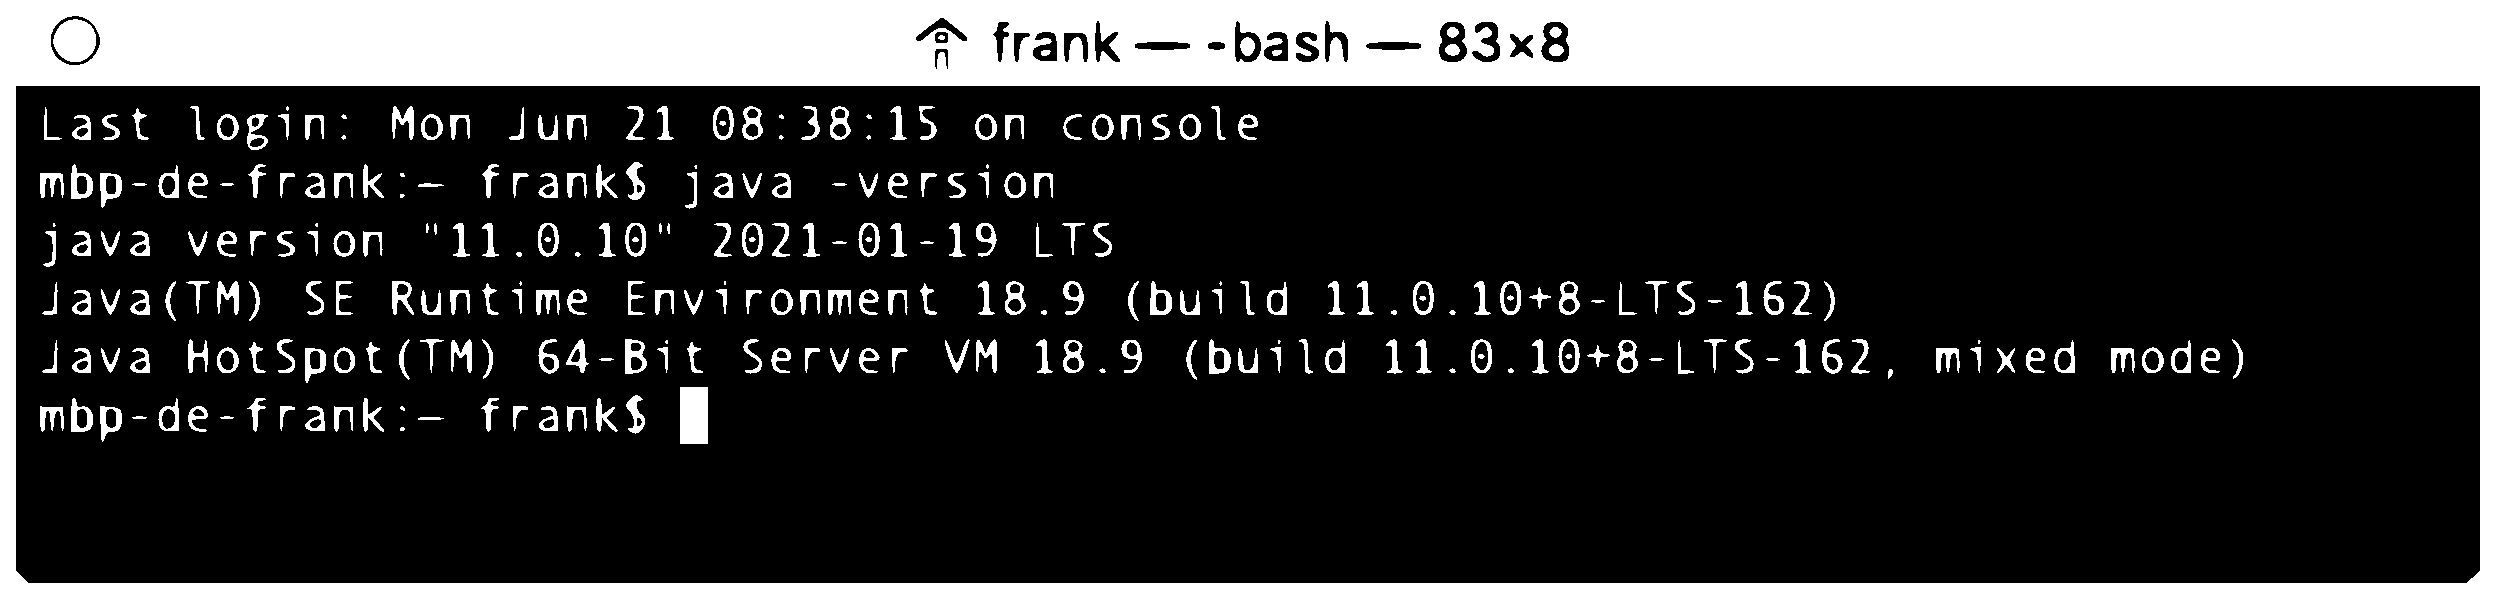
\includegraphics[scale=0.25]{images/CheckJavaVersion.eps}}
    \centering
    Also useful to see which version is installed
\end{exampleblock}


\begin{alertblock}{Do I need to install Java ?}
    \centering
    If Java command is not recognized or if version is less than 21 :\\
    \textcolor{red}{\textbf{You must install Java (again) !}}\\
    \vspace{0.5cm}
    \textbf{In this screenshot, we check Java version is at least 11}\\
    \textbf{Please update information to the latest needed JRE release}
\end{alertblock}

\end{frame}

\section{Install Java}
\subsection{Pick a Java distribution}
\begin{frame}
\begin{block}{Select one of these distros and follow installation instructions}
    \begin{itemize}
        \item \textcolor{blue}{\textbf{\underline{\href{https://adoptopenjdk.net}{AdoptOpenJDK}}}}
        \item \textcolor{blue}{\textbf{\underline{\href{https://www.azul.com/downloads/?package=jre}{Azul Zulu OpenJDK}}}}
        \item \textcolor{blue}{\textbf{\underline{\href{https://docs.aws.amazon.com/corretto/index.html}{Amazon Coretto}}}}
        \item \textcolor{blue}{\textbf{\underline{\href{https://bell-sw.com}{Liberica OpenJDK}}}}
        \item \textcolor{blue}{\textbf{\underline{\href{https://www.oracle.com/fr/java/technologies/javase-downloads.html}{Oracle Java SE}*}}}
    \end{itemize}
\end{block}
\begin{alertblock}{Java Version Alert}
    \centering
    \textcolor{red}{\textbf{Pick at least Java 21 Version}}\\
    \textbf{Prefer a Long Term Support Java Runtime Environment}\\
     \textbf{*Prefer Oracle Java SE as it is used for dev. and debug}\\
\end{alertblock}
\end{frame}


\subsection{Check Java Version}
\begin{frame}
\begin{exampleblock}{Once installation has finished : check Java Version !}
    \center{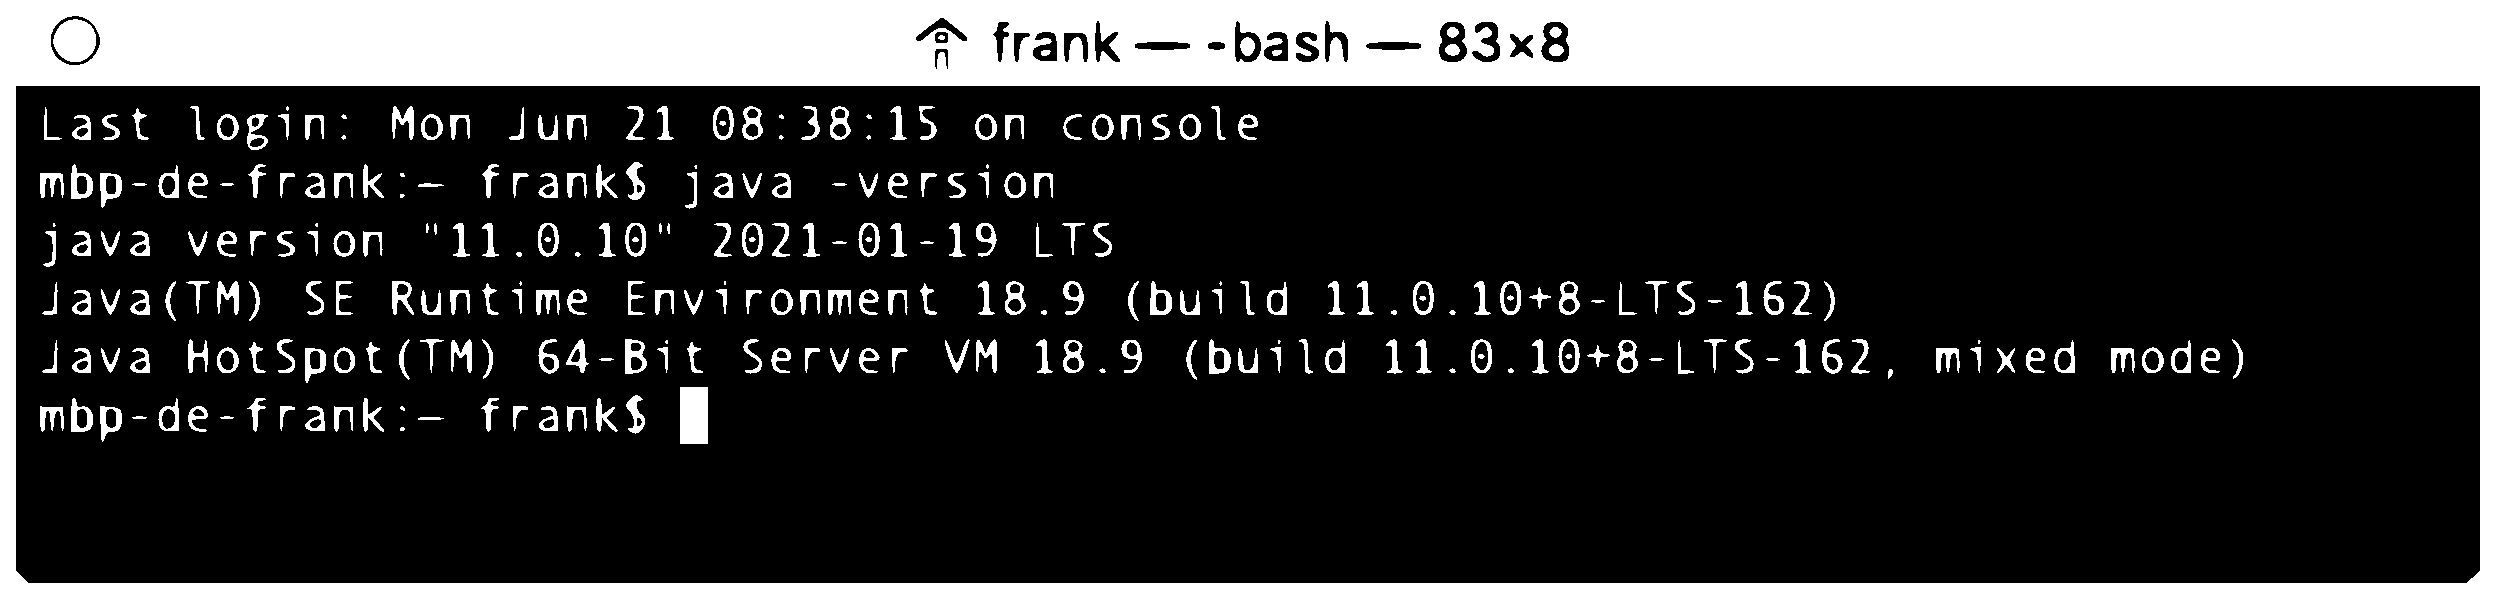
\includegraphics[scale=0.25]{images/CheckJavaVersion.eps}}
\end{exampleblock}
\centering
    \textcolor{red}{\textbf{Just to be sure Java has been properly installed !}}\\
    \vspace{0.5cm}
    \textbf{In this screenshot, we check Java version is at least 11}\\
    \textbf{Please update information to the latest needed JRE release}
\end{frame}

\section{Install Hardware}
\subsection{Available and planned Hardware}
\begin{frame}[containsverbatim]

\begin{block}{Available Hardware}
    \begin{itemize}
        \item ADWin Pro I and II
        \item ADwin Gold I and II
        \item Arduino Uno R3, R4 with support for ADS1115 (ADC 15bits)
    \end{itemize}
\end{block}

\begin{alertblock}{Planned Hardware}
    \begin{itemize}
        \item Enhanced Arduino Uno with DAC 12bits
        \item Portenta H7
        \item Teensy 4
        \item Portenta Machine Control
    \end{itemize}
\end{alertblock}
\end{frame}

\subsection{How to install ADWin ?}
\begin{frame}[containsverbatim]
\begin{block}{Overall Steps}
    \begin{itemize}
        \item Download Software
        \item Install Software
        \item Configure Hardware
    \end{itemize}
\end{block}
\end{frame}

\begin{frame}[containsverbatim]
\begin{block}{Steps to install Software}
 \begin{itemize}
        \item Follow this link to download
 \textcolor{blue}{\textbf{\underline{\href{https://www.adwin.de/pub/cd/ADwin-CD.zip}{Software}}}}
        \item Uncompress downloaded Zip file
        \item Execute Setup.exe installer
    \end{itemize}
\end{block}

\begin{alertblock}{Your platform is MacOS or Linux ?}
    In this case, there are two alternatives :
    \begin{itemize}
        \item \textcolor{blue}{Use WineHQ for OSX prior to 10.15}
        \item \textcolor{blue}{Use Docker Desktop for any OSX or Linux version}
    \end{itemize}
    \centering
    Please check DOCoMETRe help in\\Special topics of the table of contents
\end{alertblock}
\end{frame}

\begin{frame}[containsverbatim]
\begin{block}{Steps to configure Hardware}
 \begin{itemize}
        \item Run ADConfig.exe program
        \item Configure Compiler in ADBasic.exe Program
    \end{itemize}
\end{block}

\begin{exampleblock}{Hint}
 \centering \textbf{Remember there is online help in both programs !}
\end{exampleblock}

\end{frame}

\subsection{How to install Arduino Uno ?}
\begin{frame}[containsverbatim]

\begin{block}{Two Steps}
    \begin{itemize}
        \item Download Software from \textcolor{blue}{\textbf{\underline{\href{https://www.arduino.cc/en/software}{Arduino}}}}
        \item Install Software : simply uncompress downloaded file
    \end{itemize}
\end{block}

\begin{alertblock}{}
    \centering
    \textcolor{red}{\textbf{Please choose Legacy IDE or CLI version}}\\
    \textcolor{red}{\textbf{Put uncompressed file in a folder}}\\
    \textcolor{red}{\textbf{where you have all rights}}
\end{alertblock}

\end{frame}

\section{Install DOCoMETRe}
\subsection{How to install DOCoMETRe ?}
\begin{frame}[containsverbatim]
\begin{block}{Two Steps}
    \begin{itemize}
        \item Download Software from \textcolor{blue}{\textbf{\underline{\href{https://fbuloup.github.io/DOCoMETRe/}{here}}}}
        \item Install Software : simply uncompress downloaded file
    \end{itemize}
\end{block}

\begin{alertblock}{}
    \centering
    \textcolor{red}{\textbf{Put uncompressed file in a folder}}\\
    \textcolor{red}{\textbf{where you have all rights}}
\end{alertblock}

\begin{alertblock}{MacOSX Only}
    \justifying
    If you get this kind of message the first time you start the application : \textbf{"<< DOCoMETRe >> is damaged and can't be opened. You should move it to the Trash."},
    please follow this \textcolor{blue}{\textbf{\underline{\href{https://github.com/fbuloup/DOCoMETRe/wiki/Note-for-OSX-users}{link}}}} for a short
    tutorial on how to solve this problem.
    
\end{alertblock}

\end{frame}

\end{document}
